\documentclass[twocolumn,10pt]{article}
\usepackage[utf8]{inputenc}
\usepackage[T1]{fontenc}
\usepackage{lmodern}
\usepackage[margin=0.85in,top=0.9in,bottom=0.9in]{geometry}
\usepackage{amsmath,amssymb}
\usepackage{graphicx}
\usepackage{booktabs}
\usepackage{url}
\usepackage[numbers,sort&compress]{natbib}
\usepackage[hidelinks]{hyperref}
\usepackage{caption}
\usepackage{microtype}
\usepackage{xcolor}
\captionsetup{font=small,labelfont=bf}
\renewcommand{\topfraction}{0.95}\renewcommand{\bottomfraction}{0.6}\renewcommand{\textfraction}{0.05}\renewcommand{\floatpagefraction}{0.75}
\graphicspath{{figures/}}

\title{\textbf{ThinPFN: a prior-fitted network for small-sample credit scoring, trained on one desktop GPU and validated on ten public portfolios}}
\author{\textbf{Javier Mancilla Montero}\\ SquareOne Labs\\ \texttt{javier.m@squareonecap.com}}
\date{}

\begin{document}
\twocolumn[{
\maketitle
\begin{abstract}
\noindent
Tabular foundation models replace the model-per-portfolio workflow of credit scoring with a single network, pre-trained
on synthetic data, that reads a labelled table as context and scores new rows in one forward pass. We ask how much of
that capability can be reproduced, understood and owned at small scale. ThinPFN is a 25.6M-parameter prior-fitted
network pre-trained for six hours on one desktop GPU over 1.02 million synthetic tables drawn from structural causal
priors and a credit ledger simulator; no real row enters pre-training. We evaluate it on ten public credit portfolios
from four countries with a sealed test protocol: the test split of every book was read once, after the weights and the
inference recipe were frozen, with contexts of 200, 500 and 1,000 labelled rows and paired bootstrap intervals against
logistic regression, XGBoost tuned on the context, and TabPFN~v2. ThinPFN ties TabPFN~v2 on the ten-book mean
(0.697 / 0.709 / 0.727 against 0.688 / 0.710 / 0.728 at the three context sizes), is ahead of it at the smallest
context, beats tuned XGBoost in 23 of 30 cells (15 significantly, 2 significantly behind) and logistic regression in
29 of 30. Its weakness is concentrated in one regime, strong nonlinear signal, where boosted trees and the larger model
stay three to six points ahead at small contexts. Two inference-time choices made with fixed weights, quantile-normal inputs and an
average over column permutations, are worth 0.022 AUC, more than any change to the prior we tried. Code, weights, the
benchmark with split manifests, and the training recipe are released for non-commercial use.
\end{abstract}
\vspace{1.2em}
}]
\renewcommand{\thefootnote}{\fnsymbol{footnote}}
\footnotetext[1]{ThinPFN is a personal research project of the author, published from the author's GitHub account at \url{https://github.com/maximer-v/thinpfn}. The author is affiliated with SquareOne Labs.}
\renewcommand{\thefootnote}{\arabic{footnote}}\setcounter{footnote}{0}

\section{Introduction}

For more than a decade the working answer to a tabular prediction problem in credit, fraud or collections has been a
gradient-boosted tree ensemble \citep{chen2016xgboost}, fitted per portfolio, tuned per portfolio, and refitted every
time a batch of outcomes arrives. The reasons are good ones: boosted trees are cheap, fast, handle missing values and
mixed types, and their explanations are accepted by model-risk functions. Benchmarks that compare them with neural
networks on medium-sized tables keep finding them ahead or tied \citep{grinsztajn2022why,mcelfresh2023when}. The cost
of this regime is not accuracy; it is the unit of work. Every new product, segment, country or partner needs its own
model, its own validation cycle and its own retraining schedule, and the first months of a new portfolio, when a few
hundred outcomes exist, are exactly when a dedicated model is least reliable.

Tabular foundation models change the unit of work. A network is pre-trained once, on synthetic tables, to perform
Bayesian prediction in context: the labelled rows of a new problem are the prompt, the unlabelled rows are the query,
and the prediction is the posterior predictive of a prior the network has absorbed during pre-training
\citep{muller2022transformers,hollmann2023tabpfn}. No gradient step happens at decision time. A new portfolio can be
scored the day its first few hundred outcomes are known, and each confirmed outcome enters the next decision as soon as
it is appended to the context. The second generation of these models \citep{hollmann2025accurate,qu2025tabicl} reaches
or beats tuned boosting on standard benchmarks up to tens of thousands of rows.

The published models are trained with large compute budgets and released as weights. We ask a narrower and, for a
practitioner, more useful question: how much of this capability can one person reproduce, understand and own, with one
desktop GPU and a few hours of training, and does a prior built around the mechanics of credit buy anything on real
portfolios? The question matters because ownership is the point. A team that can regenerate its prior, retrain its
model and audit every line between the synthetic generator and the score has a different relationship with the model
than one that downloads weights.

This paper makes three contributions. First, a complete, small instance of a tabular foundation model, ThinPFN, with
its synthetic prior, network, pre-training recipe and inference recipe documented and released. Second, a benchmark of
ten public credit portfolios from four countries with shipped split manifests, baselines fitted on identical contexts,
paired bootstrap intervals, and a sealed test split read once. Third, a measured account of what moved the result and
what did not, including a negative one: making the synthetic stream statistically resemble real books did not help,
while depth, compute and two inference-time choices did.

\section{Background}

\paragraph{Prior-fitted networks.} A prior-fitted network (PFN) is trained on tasks sampled from a prior over
data-generating processes. Each task is a table with labelled context rows and unlabelled query rows; the network is
trained to predict the query labels given the context, by cross-entropy over millions of such tasks. Because the
training distribution is the prior, the network approximates the posterior predictive under that prior for any new
table, in one forward pass \citep{muller2022transformers}. TabPFN \citep{hollmann2023tabpfn} applied this to small
tabular classification with a prior of random structural causal models (SCMs) and Bayesian neural networks; the second
version \citep{hollmann2025accurate} added a per-cell architecture that attends across both rows and features, a richer
prior, and support for regression and larger tables. TabICL \citep{qu2025tabicl} separates column embedding, row
interaction and in-context learning into stages so that the in-context stage sees one token per row, which scales the
approach to hundreds of thousands of rows. TabDPT \citep{ma2024tabdpt} pre-trains the same kind of network on real
tables instead of a synthetic prior.

\paragraph{The ecosystem around them.} Three families of ``foundation'' approaches compete for the tabular problem in
industry. Embedding approaches train a transformer to produce a vector per row and feed that vector to a conventional
classifier; they keep the second model and its retraining. Relational foundation models operate over several linked
tables at once and are strongest where the schema itself carries signal. Single-table in-context models, the family of
TabPFN and TabICL, score directly from the labelled table and need no second model; they are the natural fit for a
scoring team whose data is already a feature table with a label. ThinPFN belongs to the third family. Its practical
promise is operational: one model per family of problems instead of per portfolio, decisions current to the latest
confirmed outcome, and the same explanation tooling (reason codes, Shapley attribution, distillation into a monotone
scorecard where regulation requires it) applied to the in-context model's scores.

\paragraph{Why synthetic priors.} The prior is the only place where domain knowledge enters a PFN. A generic SCM prior
encodes the belief that features are produced by sparse causal mechanisms with noise; it is agnostic about what the
columns mean. A domain prior can encode mechanics: that defaults arise from a delinquency process that evolves month by
month, that a bureau snapshot summarises that process with lag, that an application form measures capacity and
stability with error, and that the label is a function of the process on a horizon. Whether such mechanics transfer to
real portfolios, where the columns are whatever the lender happened to record, is an empirical question. We answer it
in Section~\ref{sec:results}.

\section{ThinPFN}

\subsection{The prior}

Every training table is generated, never collected. A table is drawn from one of three generators.

\emph{Structural causal priors.} A causal graph over $k$ latent causes and $d$ observed columns is sampled; the
mechanism is either a random multilayer perceptron with sampled depth, width, activation and noise, or a random
ensemble of decision trees with sampled depth and count. A continuous target is produced by the same mechanism and
thresholded at a sampled prevalence to give a binary label. Hyper-parameters are drawn from log-uniform ranges so that
most tables are moderately learnable and a few are hard.

\emph{Credit ledger simulator.} A portfolio is drawn: a product tag (card, instalment, peer-to-peer, vehicle; the tag
is metadata and does not change the mechanics), a prevalence between 2 and 35 percent, an observation window of three to
eleven months, a default horizon of one to twelve months, a label definition (ever 30, 60 or 90 days late, or the end
state), a thin-file share, a drift strength and noise levels. Each borrower has latent traits whose linear combination
is a risk score. A Markov delinquency chain over eleven states (no consumption, paid in full, revolving, one to eight
months late) evolves monthly; the probability of slipping one state rises with the risk score and with a smooth random
macro path, the probability of curing falls with it, and the 90-plus states are nearly absorbing. The label is one if the
chain meets the label definition within the horizon after the observation window; prevalence is matched by bisection on
the slip intercept. Observed columns are emitted in blocks, each present with its own probability: the ledger (monthly
delinquency status in the coding of the UCI Taiwan dataset, and optionally bill and payment amounts), a credit limit and
application columns (noisy monotone transforms of single traits), bureau columns (noisy monotone transforms of the risk
score), utilisation and payment ratios derived from the ledger, nominal demographic columns and an age, and an
application date when the portfolio drifts. A share of borrowers are thin files and lose the ledger block.

\emph{Drift.} With a small probability the generic tables receive a cohort index in $[0,1]$ and are generated in
cohort buckets: for the MLP prior a sparse subset of the mechanism's weights moves along the cohort; for the tree prior
each bucket draws its own tree ensemble, so the mechanism changes between cohorts rather than shifting smoothly; with
probability one half the continuous target is also tilted along the cohort (prevalence drift). The context can then be
the early cohorts and the query the late ones.

Every table passes the same contract: a random context share between 0.3 and 0.9, missing values injected completely
at random on a few columns or dependent on the value of one column, nuisance columns (noise, collinear copies, ratios),
standardisation of numeric columns on the context rows, and a learnability filter that drops tables on which an
extra-trees classifier fitted to the context scores below 0.55 or above 0.995 AUC on the query. The released mixture
is 0.40 MLP-SCM, 0.20 tree-SCM, 0.30 ledger, 0.07 drifting MLP-SCM and 0.03 drifting tree-SCM, with 256 to 1,024 rows
and up to 64 columns per table.

\subsection{The network}

ThinPFN is a per-row model. Each row becomes one token: a linear map of its standardised feature vector concatenated
with a per-cell missingness indicator and a per-column categorical flag (the released weights were trained with the
flag off), plus a learned label embedding on context rows and an ``unknown'' embedding on query rows, plus a periodic
embedding of the cohort index. Twenty-four learned ``thinking'' rows are prepended. A twelve-layer pre-norm transformer
of width 512 with eight heads runs over the rows under a mask in which context rows and thinking rows attend to each
other and to themselves, and query rows attend to the context, the thinking rows and themselves. A query row's score
therefore never depends on which other query rows are in the batch, and scoring can be batched freely. A linear head
produces two logits per row; the loss is the cross-entropy on query rows. The model has 25.6M parameters. The
column-wise and row-wise attention stages of the staged architectures \citep{qu2025tabicl} are implemented but were too
slow to train at this budget; a 3.3M per-row model with the same prior reaches the same development accuracy as the
staged model at a fraction of the cost, so the released model has no such stages.

\subsection{Pre-training}

The released weights are one run of 16,000 AdamW steps with 64 tables per step (1.02 million tables), learning rate
$5\times10^{-4}$ with 400 warm-up steps and cosine decay to zero, weight decay 0.01, gradient clipping at 1.0, bf16
autocast, and tables generated on the fly by twelve CPU workers. The run took six hours on a single desktop GPU with
unified memory; it is bound by table generation, not by the network, which holds five gigabytes. A fixed held-out
synthetic batch is scored every fifty steps; the last six snapshots, 500 steps apart, are averaged into the released
weights. The real-book development AUC tracked the held-out synthetic loss throughout (Figure~\ref{fig:training}),
which is the practical signal that the prior is being fitted rather than memorised.

\begin{figure}[t]
\centering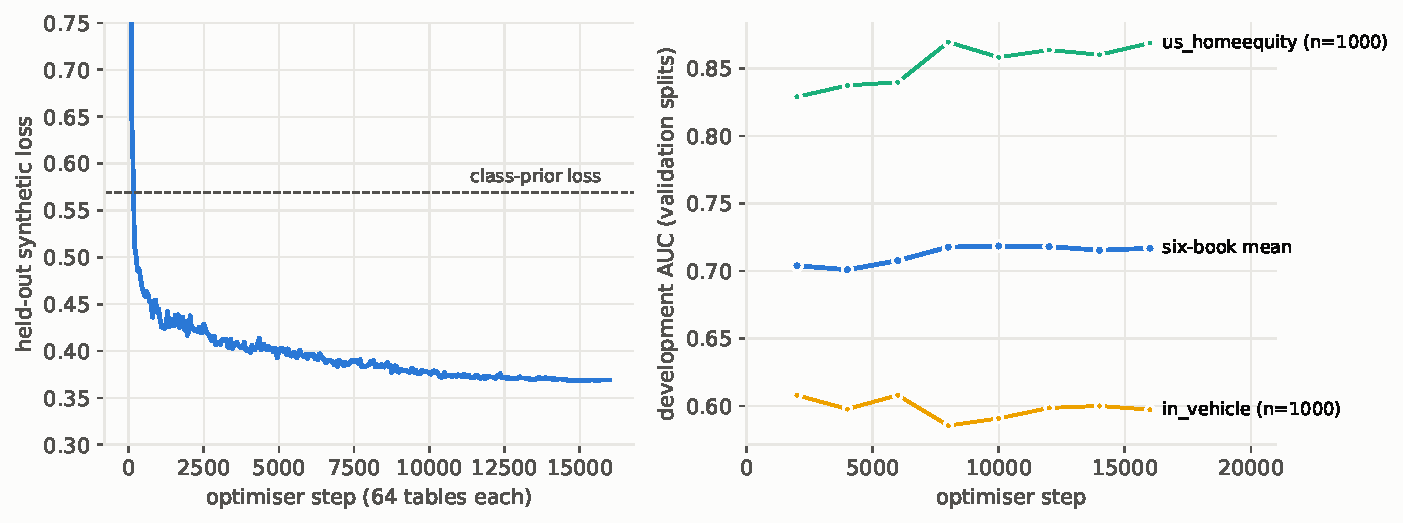
\includegraphics[width=\linewidth]{training.pdf}
\caption{Pre-training. Left: loss on a fixed held-out synthetic batch against the class-prior loss it must beat. Right:
development AUC (validation splits, never the test split) on the six charter books, with the two books that moved most.}
\label{fig:training}
\end{figure}

\subsection{Inference}
\label{sec:inference}

Two choices made after pre-training, on validation splits and with the weights fixed, define the released inference
recipe. First, numeric columns are transformed to a quantile-normal scale fitted on the context rows, instead of the
z-score clipped at four standard deviations that the prior was standardised with. Real credit columns are heavy-tailed
and discrete (half the columns of the benchmark books have fewer than six percent distinct values; money columns carry
point masses); the z-score squashes most of their rows into a narrow band while the prior's own inputs are close to
Gaussian. Second, the log-odds are averaged over eight random column orders. The row embedding is a slot-wise linear
map, so the network is not permutation-invariant over columns, and the orders act as a cheap ensemble. On the 3.3M
development model the two changes together are worth 0.022 AUC on the ten-book mean, with no cell significantly worse
(Figure~\ref{fig:inference}); the released model inherits both.

\begin{figure}[t]
\centering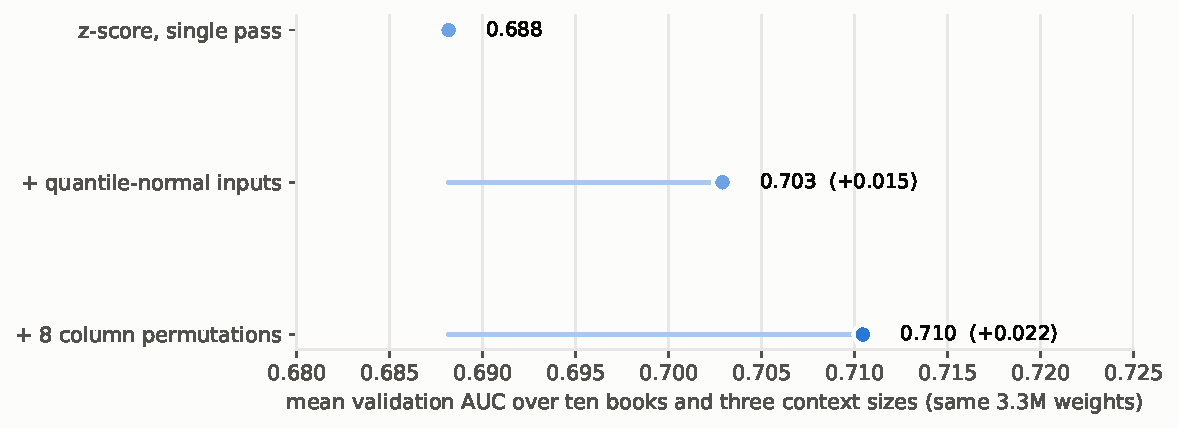
\includegraphics[width=\linewidth]{inference.pdf}
\caption{Inference recipe on fixed weights (3.3M development model, validation splits, ten books, three context sizes).}
\label{fig:inference}
\end{figure}

\section{Benchmark}

\paragraph{Books.} Ten public consumer-credit portfolios with a binary default label (Table~\ref{tab:books}). Six form
the charter set the study was designed around; four were added for breadth from lenders in the United States, China and
India. Two pairs share an origin (the two Taiwan views; the two LendingClub extracts, from different periods and with
different fields; the two Taiwan views share their 4,500 test rows), so the set contains eight source datasets. Each
book carries a frozen four-way split into training, validation, calibration and test rows; two books with origination
dates (LendingClub, Prosper) are split out of time, the rest at random with stratification. The two Taiwan books are
behavioural scoring (six months of repayment history, label the next month); the other books use origination-time
fields, with fields observed after origination (payments received, recoveries, current balance) excluded, and PPDai's
29 fields taken as released. String columns are ordinal-coded on the whole source table (label-free), a transductive
step the sealed test inherits. TVS contains many identical feature rows across splits (1,919 of the test rows match a
training row exactly); the bootstrap unit is the row everywhere. The repository ships the split manifests keyed to the
rows of the public source files, whose hashes are recorded, and a preparation script that rebuilds every table.

\begin{table*}[t]
\centering\small
\caption{The ten books. Rows are those used after the split rules; prevalence is of the test split; OOT = out-of-time splits by origination date.}
\label{tab:books}
\begin{tabular}{llrrr}
\toprule
book & origin & rows & feat. & prev. \\
\midrule
uci\_full & UCI 350, Taiwan cards, 2005 & 30,000 & 23 & 0.22 \\
tw\_cards & same table, 4,000 training rows & 16,000 & 23 & 0.22 \\
us\_bureau & Give Me Some Credit, US & 9,335 & 10 & 0.06 \\
in\_vehicle & L\&T vehicle loans, India & 9,335 & 19 & 0.22 \\
us\_homeequity & HMEQ home equity, US & 5,960 & 12 & 0.20 \\
us\_p2p & LendingClub 2007 to 2015 & 7,832 & 13 & 0.16 \\
lending\_club & LendingClub 2007 to 2015 vintages, OOT & 642,138 & 28 & 0.15 \\
ppdai & PPDai, China & 55,596 & 29 & 0.13 \\
prosper & Prosper 2005 to 2014, OOT & 38,907 & 36 & 0.15 \\
tvs & TVS Credit cross-sell, India & 119,528 & 29 & 0.02 \\
\bottomrule
\end{tabular}
\end{table*}

\paragraph{Protocol.} For each book and each context size $n \in \{200, 500, 1000\}$, three contexts are drawn from the
training split with stratified sampling (seeds 0, 1, 2). Every model scores the same query rows (the evaluation split,
subsampled to 4,000 rows when larger) from the same context. The metric is ROC AUC, averaged over the three seeds. The
difference between ThinPFN and each baseline carries a 95\% paired bootstrap interval over the query rows (1,000
resamples, seeds averaged inside each resample); a cell is ``significant'' when the interval excludes zero.

\paragraph{Baselines.} Logistic regression with median imputation and standardisation. XGBoost with a small grid of
depth, learning rate and regularisation chosen on a held-out slice of the context with early stopping, which is how a
practitioner would tune it with this little data; at $n < 300$ a fixed shallow configuration is used. TabPFN~v2
\citep{hollmann2025accurate} with its released weights and default settings.

\paragraph{Sealed test.} Development used validation splits only, many times. The test split of every book was read
once, by a dedicated script, after the released weights and the inference recipe were frozen. Three claims were written
before that read: G2, the original gate of the study, that ThinPFN beats both TabPFN~v2 and XGBoost on the six charter
books with the interval above zero on at least four and never significantly behind; C1, that at $n=200$ it is
significantly ahead of both on at least four of six; and C2, that the ten-book mean is within 0.01 of TabPFN~v2 at
$n=500$ and $n=1000$. The results below report all three.

\section{Results}
\label{sec:results}

\begin{table}[t]
\centering\small
\caption{Sealed test: mean ROC AUC over ten books.}
\label{tab:main}
\begin{tabular}{lcccc}
\toprule
$n$ & ThinPFN & TabPFN v2 & XGBoost & Logistic \\
\midrule
200 & \textbf{0.697} & 0.688 & 0.654 & 0.654 \\
500 & 0.709 & 0.710 & 0.674 & 0.665 \\
1000 & 0.727 & 0.728 & 0.706 & 0.679 \\
\midrule
\multicolumn{5}{l}{\footnotesize Cells ahead of 30 (sig.\ ahead / behind): TabPFN v2 17 (7/5),} \\
\multicolumn{5}{l}{\footnotesize XGBoost 23 (15/2), logistic 29 (23/0)} \\
\bottomrule
\end{tabular}
\end{table}

\begin{figure}[t]
\centering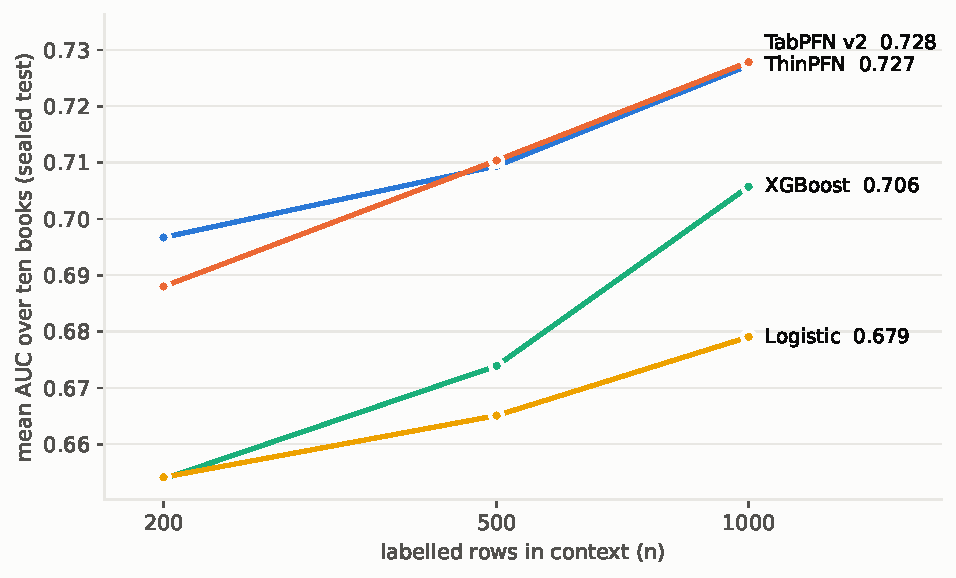
\includegraphics[width=\linewidth]{mean_auc.pdf}
\caption{Sealed test: mean AUC over the ten books against context size.}
\label{fig:mean}
\end{figure}

\begin{figure*}[t]
\centering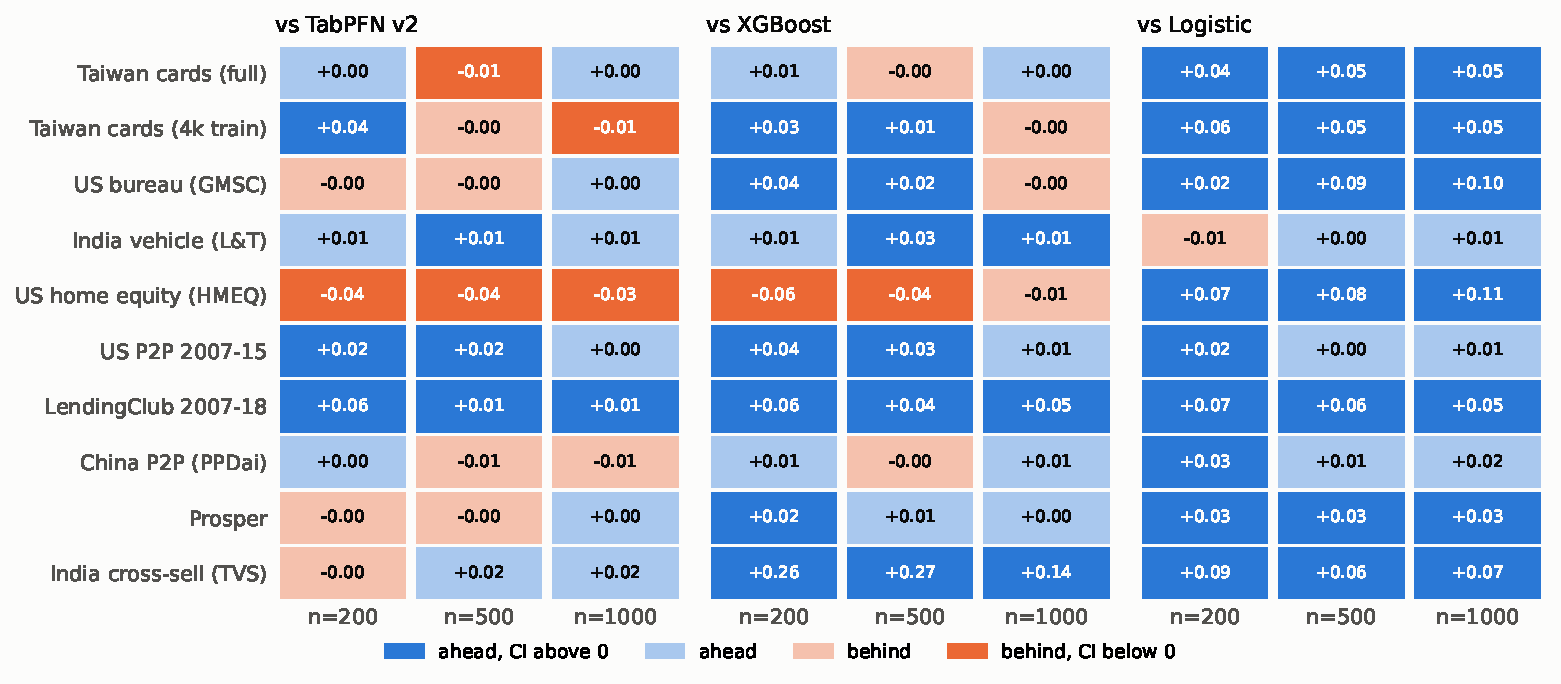
\includegraphics[width=0.95\textwidth]{cells_grid.pdf}
\caption{Every cell of the sealed test. Colour: sign of the AUC difference of ThinPFN against the baseline, saturated
when the 95\% paired bootstrap interval excludes zero.}
\label{fig:grid}
\end{figure*}

\paragraph{Main result.} Table~\ref{tab:main} and Figure~\ref{fig:mean} give the ten-book means. ThinPFN ties TabPFN~v2
on the mean, is ahead of it by 0.009 at $n=200$ and within 0.001 at the two larger contexts, and is ahead of tuned
XGBoost by 0.043, 0.035 and 0.021. Against logistic regression it is ahead in 29 of 30 cells (the exception is
in\_vehicle at $n=200$, $-0.010$). C2 passes. G2 and C1 fail: at
$n=200$ the interval is above zero against both baselines on two of the six charter books (tw\_cards and us\_p2p), not
four, and one charter book is significantly behind both. ThinPFN does not have a decisive win over TabPFN~v2; it has
parity at a training budget of six desktop GPU-hours, a small-context advantage on several books,
and a documented failure mode.

\paragraph{Per book.} Figure~\ref{fig:grid} shows every cell. The significant wins over TabPFN~v2 at $n=200$ are
LendingClub ($+0.062$), tw\_cards ($+0.038$) and us\_p2p ($+0.016$); in\_vehicle is ahead at every $n$ but significant
only at $n=500$. The losses are concentrated in one book, us\_homeequity, at $-0.039$, $-0.038$ and $-0.028$, which is
also the only book where XGBoost is significantly ahead of ThinPFN. The remaining significant losses to
TabPFN~v2 are uci\_full at $n=500$ ($-0.009$) and tw\_cards at $n=1000$ ($-0.013$). The XGBoost comparison carries a
caveat: on TVS (2 percent prevalence, four positives in a 200-row context) the small-context XGBoost configuration
collapses to a constant score for every seed at $n=200$ and one seed at $n=500$, so those cells (AUC 0.50) inflate the
count; excluding TVS, ThinPFN is ahead of XGBoost in 20 of 27 cells (12 significantly, 2 significantly behind), with
mean differences of $+0.019$, $+0.009$ and $+0.008$. On the three weak-signal books, where no model reaches 0.66 AUC
(in\_vehicle, ppdai, us\_p2p), ThinPFN is ahead of TabPFN~v2 in seven of nine cells and of XGBoost in eight of nine.

\paragraph{What explains the losses.} On the development splits, ThinPFN's deficit to TabPFN~v2 at $n=1000$ correlates
$-0.87$ with the book's achievable AUC (a tuned boosting model on the full training split), $-0.73$ with the AUC of the
single best feature, and $-0.69$ with the nonlinearity gap (boosting minus logistic). The model regularises well where
there is little to find and under-exploits strong nonlinear structure. us\_homeequity has a nonlinearity gap of 0.13,
the largest in the set; a twelve-layer per-row network reaches 0.89 there where the larger model reaches 0.92. The
development evidence below, where the gains from a deeper and longer-trained model landed on exactly these books,
points to network capacity rather than to the prior; since that comparison changed depth and training budget together,
capacity is the working hypothesis, not an established cause.

\subsection{What moved the result during development}

Four findings from the validation splits, reported here because they are the transferable part of the work. The
prior ablations were run at equal compute (3.3M model, 160k tables); the size comparison was not. The development
record behind them (realism audit, leave-dataset-out runs, prior ablations) is summarised rather than released; the
released result files are the sealed test, the inference study and the size comparison.

\emph{Depth and compute.} With the same prior and the same inference recipe, a 3.3M model trained on 160k tables
reaches 0.700 / 0.712 / 0.724 on the ten-book validation mean; the released 25.6M model on 1.02M tables reaches
0.706 / 0.721 / 0.737 (Figure~\ref{fig:scale}). The gain is concentrated on clean, strongly nonlinear books
(us\_homeequity at $n=1000$: 0.848 to 0.904) and costs under a point on the weakest book. Within every run, the real-book
AUC followed the synthetic held-out loss, so the lever is fitting the prior better. The released run was under-driven
(gradient norms of 0.1 to 0.2 against a clip of 1.0, at half the learning rate of the small model); a higher learning
rate is the first untested training lever.

\begin{figure}[t]
\centering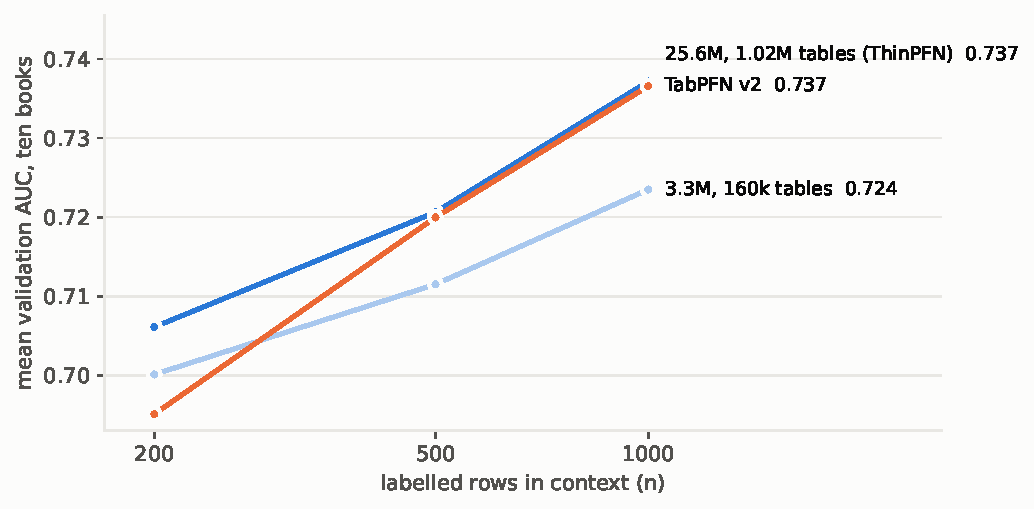
\includegraphics[width=\linewidth]{scale.pdf}
\caption{Same prior, same inference recipe, two model sizes (validation splits).}
\label{fig:scale}
\end{figure}

\emph{Statistical realism of the prior did not help.} An audit of 25 per-table statistics on 330 real tables against
the synthetic stream showed the stream far from real books on every axis (labels too predictable, columns too
continuous, too few categoricals, too symmetric). A second simulator with product and feature families and realistic
marginals, plus discretisation and prevalence-preserving label noise applied to every component, brought the stream
within noise of real books on most statistics (a leave-dataset-out discriminator fell from 0.997 to 0.909). Trained at
equal compute, the model was worse on the mean at every $n$ and significantly worse on four to six of ten books. Label
noise in training appears to teach the network to trust the context less, which hurts at larger $n$. The prior that
works is the simple one, and the lever against mismatch is on the inference side (Section~\ref{sec:inference}).

\emph{Real rows in the training stream hurt.} Mixing sub-tables of the public books (never the held-out lender) into
the stream, or copula twins of them, or a field-type vocabulary through which knowledge could transfer across lenders,
failed to beat the synthetic-only model on an unseen lender in nine of nine leave-dataset-out runs. At this scale, real
data belongs in evaluation, not in pre-training.

\emph{The ledger component is a trade.} At equal compute, a generic-only prior beat the released mixture on the Taiwan
books (uci\_full at $n=1000$: $+0.015$) and lost on the weakest book (in\_vehicle: $-0.02$). The credit mechanics buy
the weak-signal edge and cost clean-book accuracy; the weight is a choice, not a free parameter.

\section{Limitations and intended use}

ThinPFN is for the small-sample regime: contexts of 200 to a few thousand rows and at most 64 numeric or ordinal
features, binary labels. It was pre-trained on tables of at most 1,024 rows and stops improving above a few thousand
context rows, where a tuned boosted model with all the data is the better tool. On books with strong nonlinear signal
it trails TabPFN~v2 by three to four points and XGBoost by four to six points at $n \le 500$. The inference recipe and the depth were chosen on
validation splits that were read many times; the sealed test was read once, and the significant wins over TabPFN~v2 at
$n=200$ shrank from five books on validation to three on test, which is the expected size of that selection effect. The
released weights are one pre-training seed; variance across seeds has not been measured. The model is released for
research and non-commercial use; automated decisions about people require, independently of the model, a fairness
assessment, human review and the explanation tooling the lender's regulation demands.

\section{Reproducibility}

The repository contains the package (prior, network, trainer, scikit-learn style front end), the released weights (fp16,
51 MB), the benchmark with split manifests and a preparation script that rebuilds every book from its public source,
the sealed-test script and its output, the figure script, tests, and a walkthrough notebook. The pre-training command
that produced the released weights is one line; the benchmark is two. The sealed-test numbers, the inference study,
the size comparison and the training log are in \texttt{benchmark/results/}; the other development findings are
reported from the development record. A resumed training run restarts the synthetic streams, so only an uninterrupted
run reproduces the released weights exactly. The datasets keep the terms stated at their sources; one (Prosper) has no
stated licence and is used for evaluation only.

\bibliographystyle{plainnat}
\bibliography{references}
\end{document}
